%开普勒第二定律的证明

\pentry{开普勒第二定律\upref{Keple}, 角动量守恒(单个质点)\upref{AMLaw1}}
\begin{figure}[ht]
\centering
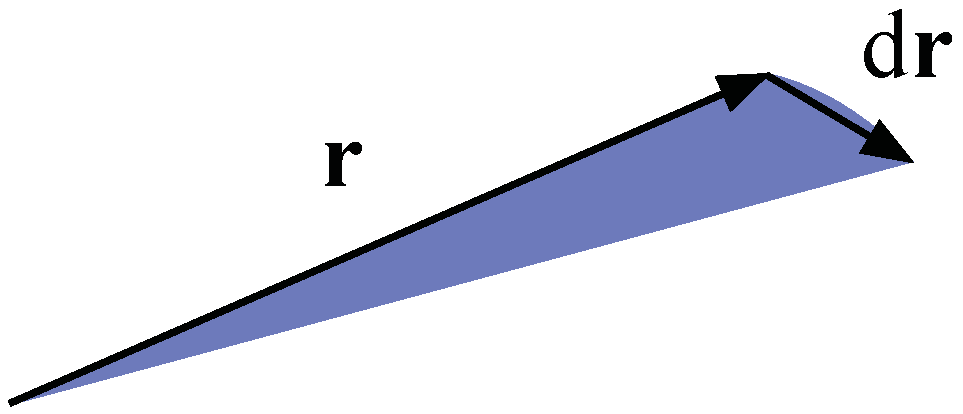
\includegraphics[width=4.5cm]{./figures/Keple21.pdf}
\caption{微小时间 $\dd{t}$ 扫过的面积} \label{Keple21}
\end{figure}

令行星的位矢为 $\vec r$,  在很小一段时间 $\dd{t}$ 内移动了 $\dd{\vec r}$,  于是扫过的面积就是以 $\vec r$ 和 $\dd{\vec r}$ 为两条边的三角形的面积 $\dd{S} = \abs{\vec r} \abs{\dd{\vec r}} \sin \theta /2 $,  其中 $\theta $ 为两条矢量的夹角.若把面积看成矢量, 方向垂直于三角形所在的平面, 则根据叉乘的定义有 $\dd{\vec S} = \vec r \cross \dd{\vec r/2}$. 两边除以 $\dd{t}$,  得扫过面积的速率为
\begin{equation}
\dv{\vec S}{t} = \frac{1}{2}\vec r \cross \dv{\vec r}{t} = \frac 12 \vec r\cross \vec v
\end{equation}
由“角动量守恒\upref{AMLaw1}”, 行星角动量不变.
$\vec r \cross (m\vec vs) = \vec L$ (常矢量, 垂直运动平面) 所以 $\dv*{\vec S}{t} = \vec L /2m$ 也是常矢量.写成标量形式, 即
\begin{equation}
\dv{S}{t} = \frac{L}{2m}
\end{equation}
所以从任意时刻 $t_0$ 开始, 在一段时间 $\Delta t$ 内行星扫过的面积为 
\begin{equation}
\begin{aligned}
\Delta S = \frac{L}{2m}\Delta t
\end{aligned}
\end{equation}
只和时间间隔有关, 而与起始位置无关.

